\begin{section}{UFO Web}

\subsection{Web Service}

Um Interoperabilitaet zwischen unterschiedlichen Programmiersprachen zu gewaehrleisten und die Spezifikation zu erfuellen wurde ein SOAP basierter Web Service in C\# realisiert. 

Der Web Service aus der 2. Ausbaustufe wurde in ein eigenes Assembly migriert und fuer die Kommunikation mit der JSF / Java Umgebung wurde ein eigenes UFO.Web Assembly angelegt. Dieses wurde im Vergleich zur zweiten Ausbaustufe nicht mit WCF, sondern laut Angabe mit dem klassischen WebSerice Basisklassen und Attributen umgesetzt. 

Die Trennung dieser zwei Dienste ermoeglicht eine unabhaengige Operation von Service bedingten Diensten als auch Web basierten Diensten. Die Umsetzung der WCF basierten Loesung wird weiterhin als Self-Hosting Ausfuehrung angeboten. Die neue Implementierung fuer die UFO.Web Weiterentwicklung der 3. Ausbaustufe wird auf einem Microsoft IIS (Internet Information Service) Server betrieben. Dies ermoeglicht auch Kompatibilitaeten zu anderen Plattformen oder Diensten, wie beispielsweise Azure.

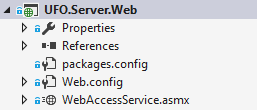
\includegraphics[angle=0, scale=0.45]{./img/3_ausb_assembly.PNG}
\FloatBarrier

Um die SOAP basierten Dienste anbieten zu koennen muessen die Business Logik Klassen via Reflection geladen werden, aehnlich zu den DAL Klassen aus der 2. Ausbaustufe. Da eine flexible Konfiguration gefragt ist ohne Code umschreiben zu muessen, werden alle relevanten Parameter in eine eigene Konfigurationsdatei eingetragen, welche beim Deployment mitgeliefert wird. 

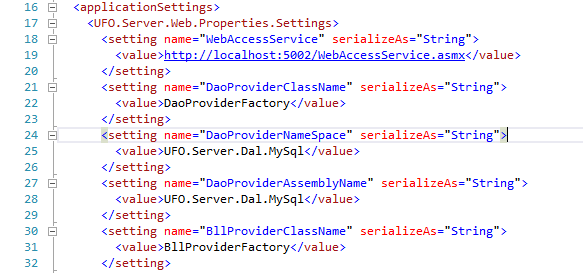
\includegraphics[angle=0, scale=0.45]{./img/3_ausb_config.PNG}
\FloatBarrier

Die Parameter werden auf dem IIS mit-deployed und referenzieren die DAL, BLL und WS relevanten Assemblies welche zur Laufzeit geladen werden. 

Um ein WSDL-Schema generieren zu koennen wird die WebAccessService Klasse, welche als Schnittstellen nach außen dient, mit den entsprechenden Attributen annotiert.

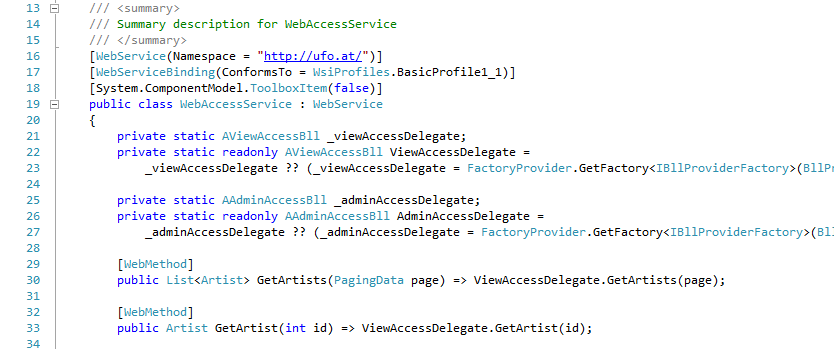
\includegraphics[angle=0, scale=0.45]{./img/3_ausb_webservice.PNG}
\FloatBarrier

Anbei eine Uebersicht der verfuegbaren WS-Methoden:

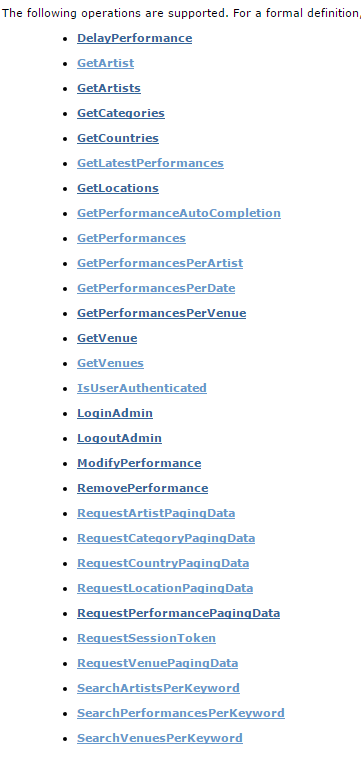
\includegraphics[angle=0, scale=0.45]{./img/3_ausb_ws_methods.PNG}
\FloatBarrier

\subsection{JSF}

Für die Entwicklung der JSF basierten Applikation wurden folgende Komponenten / Frameworks herangezogen:

\begin{itemize}
	\item PrimeFaces (fuer Ajax basierte Client / Server Kommunikation)
	\item Bootstrap (fuer die UI Anpassung)
	\item JAX-WS (fuer die Client-Klassen Generierung)
	\item Java-Beans (fuer die Datenverwaltung)
\end{itemize}

Da auch diese Applikation moeglichst hohe flexibilitaet ausweisen soll, wurde ein Abstraktionsschicht fuer die domaenenspezifischen Aufrufe erstellt in Form von einer Delegate Klasse (UfoDelegate). Die UfoDelegate Klasse besitzt eine Web Service Implementierung UfoWebService. Die Konfiguration der konkrete UfoDelegate Implementierung wird in im web.xml Deploymentdeskriptor hinterlegt. Somit ist es moeglich alternative Dienste zur Realisierung des UFO.Web Projekts aufzugreifen. Die Generierung der Klassen wurde in ein eigenes package verlegt. Alternative Implementierungen muessten nur im selben Namensraum angefuert werden. Ansonsten koennen alle bestehenden Klassen, welche auf dem Delegate aufsetzten wie gehabt verwendet werden. 

\subsection{Konzept}

Es werden .xhtml-Dateien fuer die Realisierung der Views mit JSF verwendet. Damit die Basisstruktur der Seite nicht mehrfach kopiert und redundant implementiert wird, wurde ein Template der Seitenstruktur erstellt. Die basicTemplate-Datei deklariert die Position des Headers, Content und Footers. Um auf die Daten der Business Logik zugreifen zu koennen, werden Java-Beans verwendet. 

\subsubsection{Seiten-Navigation}

Um dem Benutzer der Website eine gute User-Experiance bieten zu koennen, wurde zusaetzlich zur herkoemmlichen Navigation eine Such-Moeglichkeit angefuegt. Diese bietet auch Auto-Completion, welche nach Ort, Kuenstler und Spielstaetten operiert. Der Aufbau der Hauptseite beinhaltet eine Ansicht der aktuellsten Auffuehrungen und offeriert die Moeglichkeit nach Datum vorhergehende Auffuehrungen nachzuschlagen.

Es steht dem Benutzer auch zur Auswahl, Kuenstler in einer Listenform aufzusuchen und Details ueber diesen Kuenstler zu erfragen.

Als dritter Navigationspunkt fungiert die Uebersicht der Spielstaetten, wo alle hinterlegten Spielstaetten abgefragt werden. 

Alle Seiten besitzen querverweise auf Detailansichten bzw. besitzen Zusammenfassungen, welche Auflistungen der aktuellen Auffuehrungen darstellen. 

\subsubsection{Mock-Up}

Um eine Uebersicht der Seitendarstellung zu bekommen, wurde im Vorfeld ein Mock-Up designed.

Hauptseite: \\
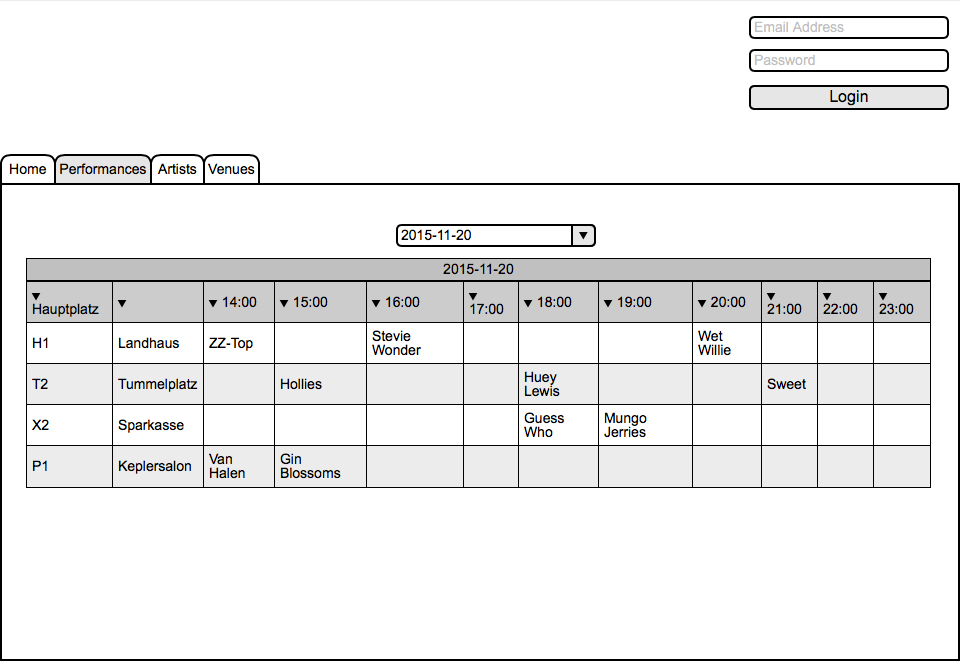
\includegraphics[angle=0, scale=0.35]{./img/performanceview.jpg}
\FloatBarrier

Artist Detail Ansichtsseite: \\
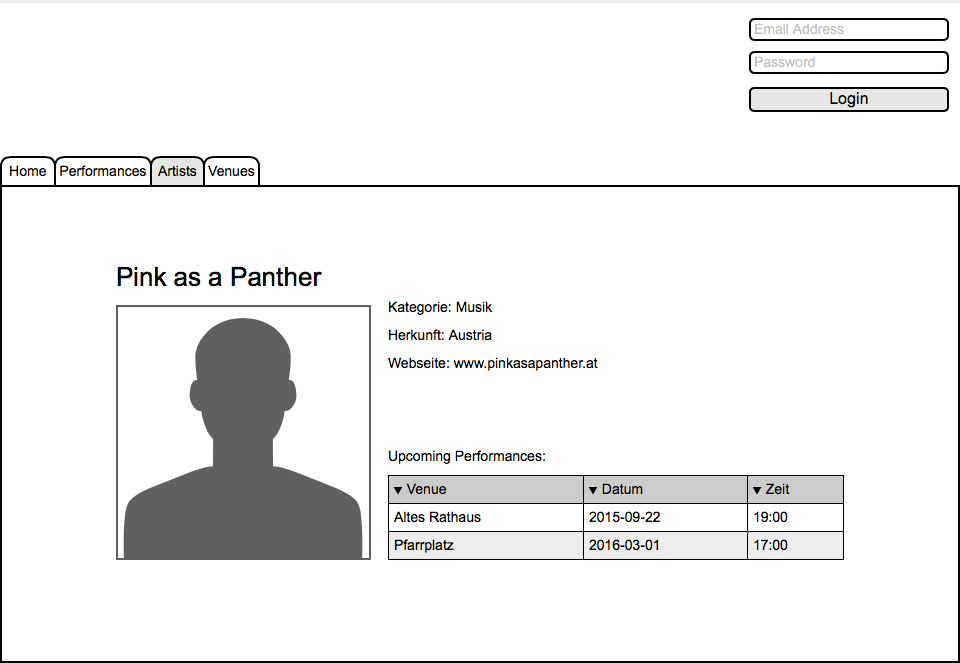
\includegraphics[angle=0, scale=0.35]{./img/artistdetailview.jpg}
\FloatBarrier


\subsection{Implementierung}

Fuer das Session-Handling wurde ein Session Bean angelegt, welches die momentane Login-Session fuer den jeweilen Benutzer beinhaltet. Dieses wird verwendet umd Editier-Funktionalitaeten anzubieten, da Auffuehrungen verschoben bzw. storniert werden koennen. Die Referenzierung dieses Beans wird von weiteren Beans via Dependency-Injection aufgeloest. Um die Benutzerdaten sicher uebertragen zu koennen, werden diese via MD5 Verschluesselung bereits am Client ge-hasht und in weiterer folge via eines SessionTokens uebermittelt. Dieser SessionToken dient auch zur Verifizierung des Benutzers, sollte dieser Aenderungen vornehmen wollen.


Da mehrfach Listings von Kuenstlern bzw. Spielstaetten gefordert sind und die Aufrufe eines Web-Services gewisse Datenlimitierungen aufweisen, wurde ein Pageing aufruf realisiert. Somit werden in dedizierten Paketen die Daten an den Client uebermittelt.

Eines der wichtigsten Beans ist das PerformanceCollectionBean, wo alle Auffuehrungen verwaltet werden. Um eine tabellarische Darstellung der Auffuehrungen anzeigen zu koennen muessen im Vorfeld diverse Gruppierungen durchgefuehrt werden. Da JSF und Primefaces keine native Gruppierung unterstuetzt wurde ein Hilfsobject PerformanceGroup entwickelt, welches zuerst nach Datum, dann Spielstaetten und anschliessend nach Auffuehrungen sortiert. Die Abbildung der PerformanceGroup ist als Map<Date, PerfromanceGroup> realisiert worden. 

Gruppierung der Performances: \\
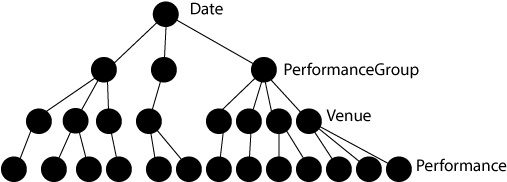
\includegraphics[angle=0, scale=0.65]{./img/tree.jpg}
\FloatBarrier

\subsection{Design und Realisierung}

Anbei werden Screen-Shots der fertiggestellten Website angezeigt: \\

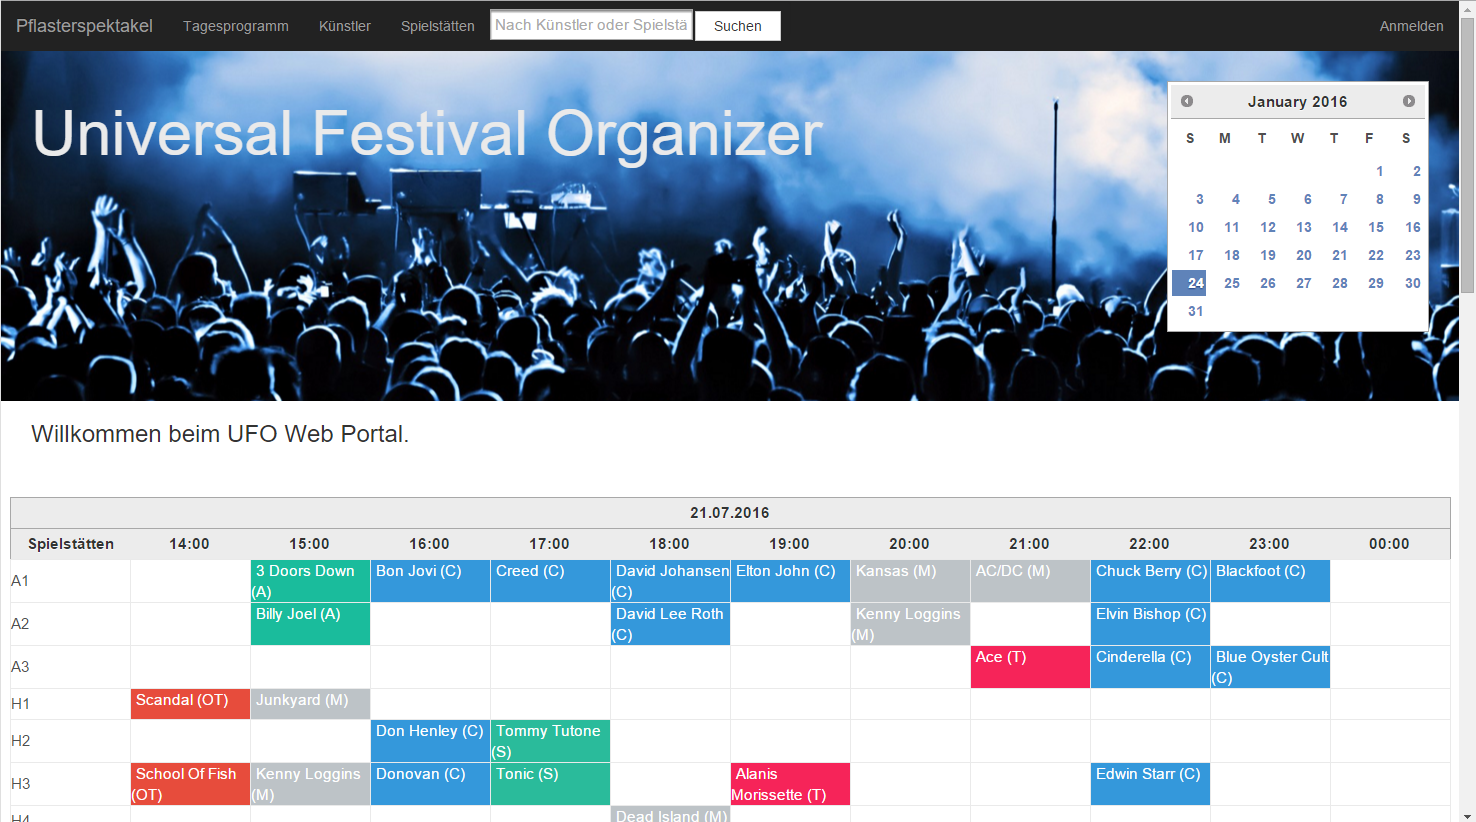
\includegraphics[angle=0, scale=0.40]{./img/3_ausb_page1.PNG}
\FloatBarrier
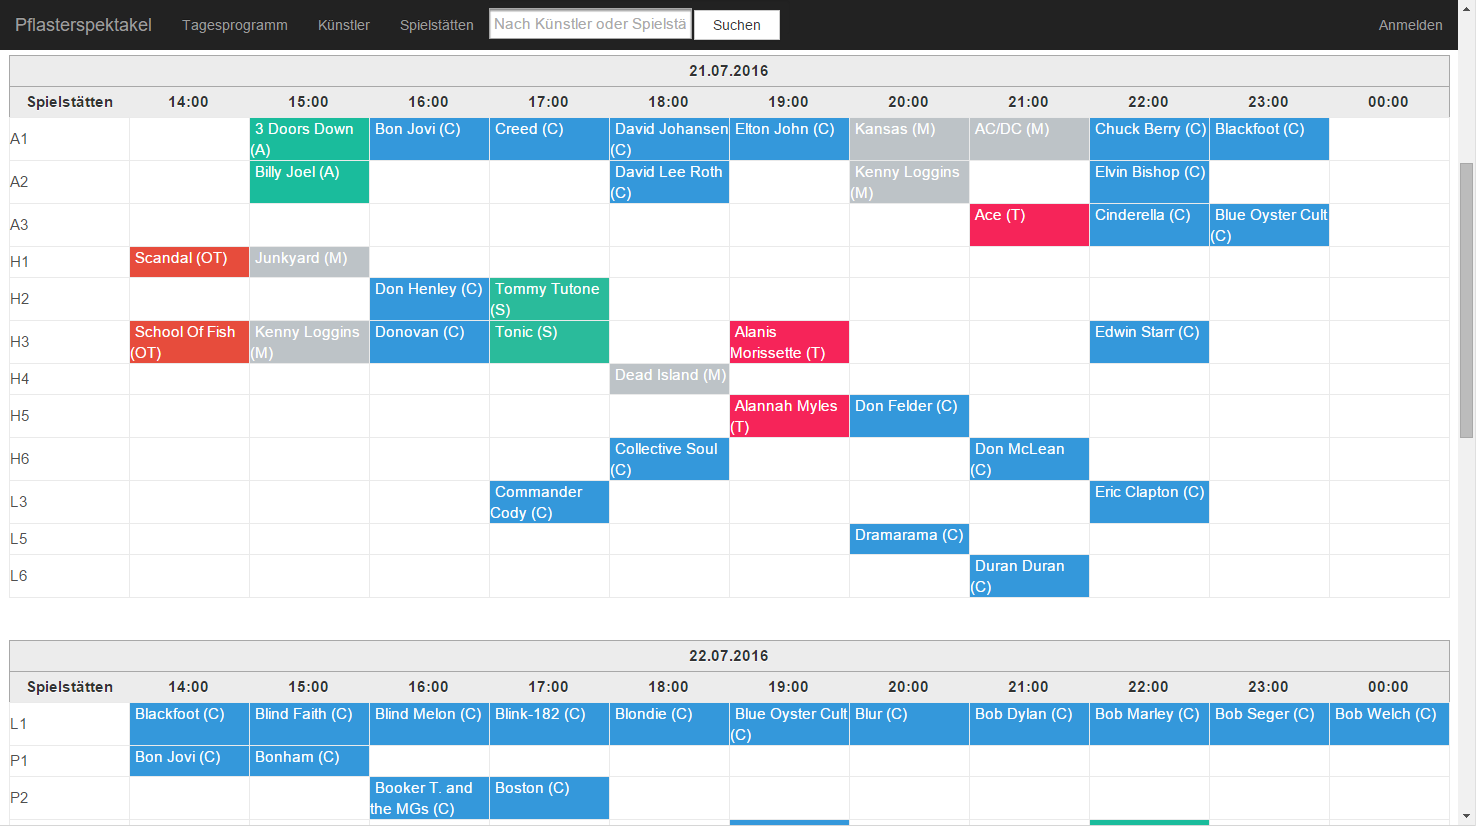
\includegraphics[angle=0, scale=0.40]{./img/3_ausb_page2.PNG}
\FloatBarrier
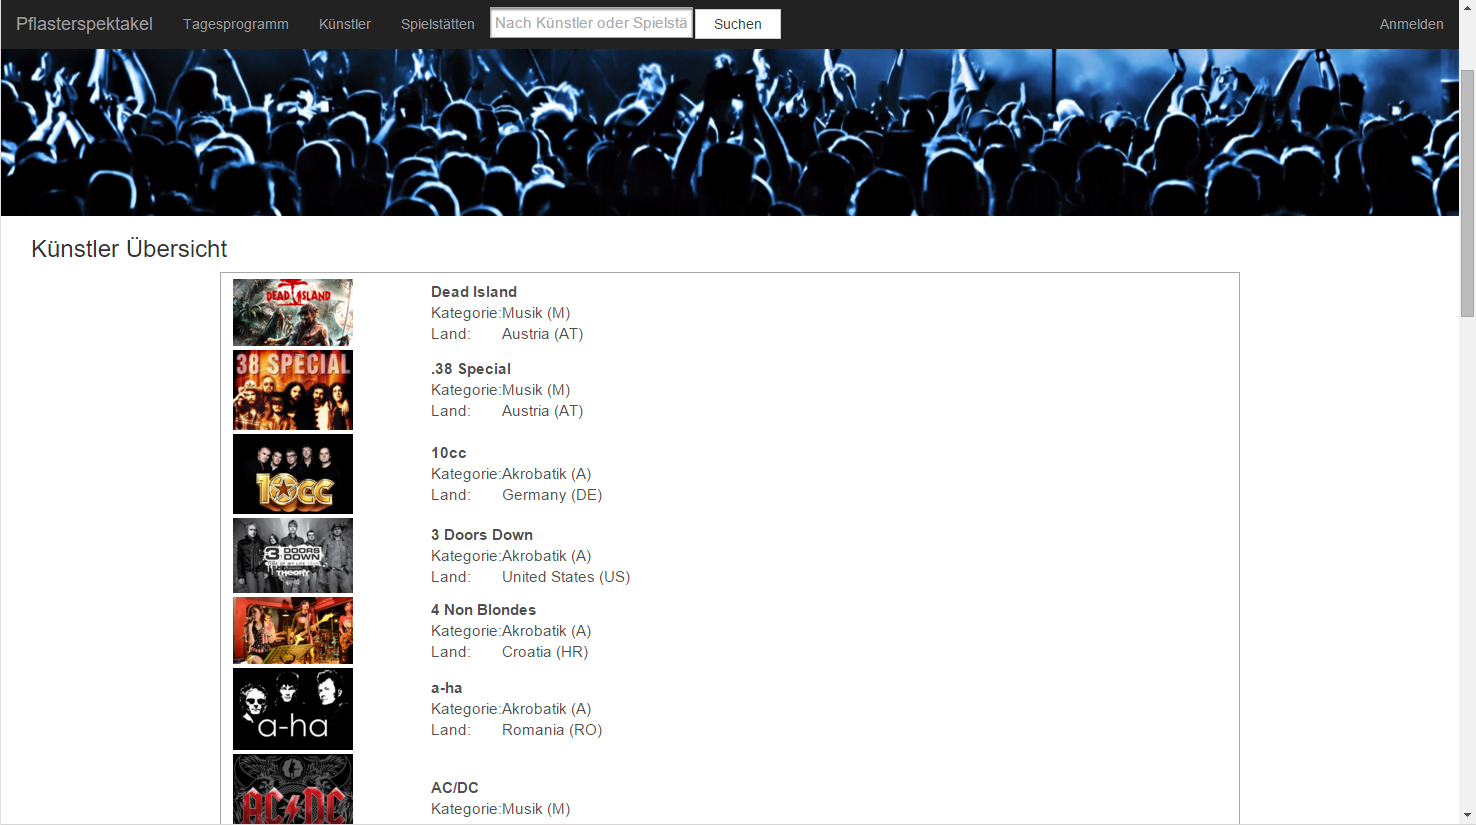
\includegraphics[angle=0, scale=0.40]{./img/3_ausb_page3.PNG}
\FloatBarrier
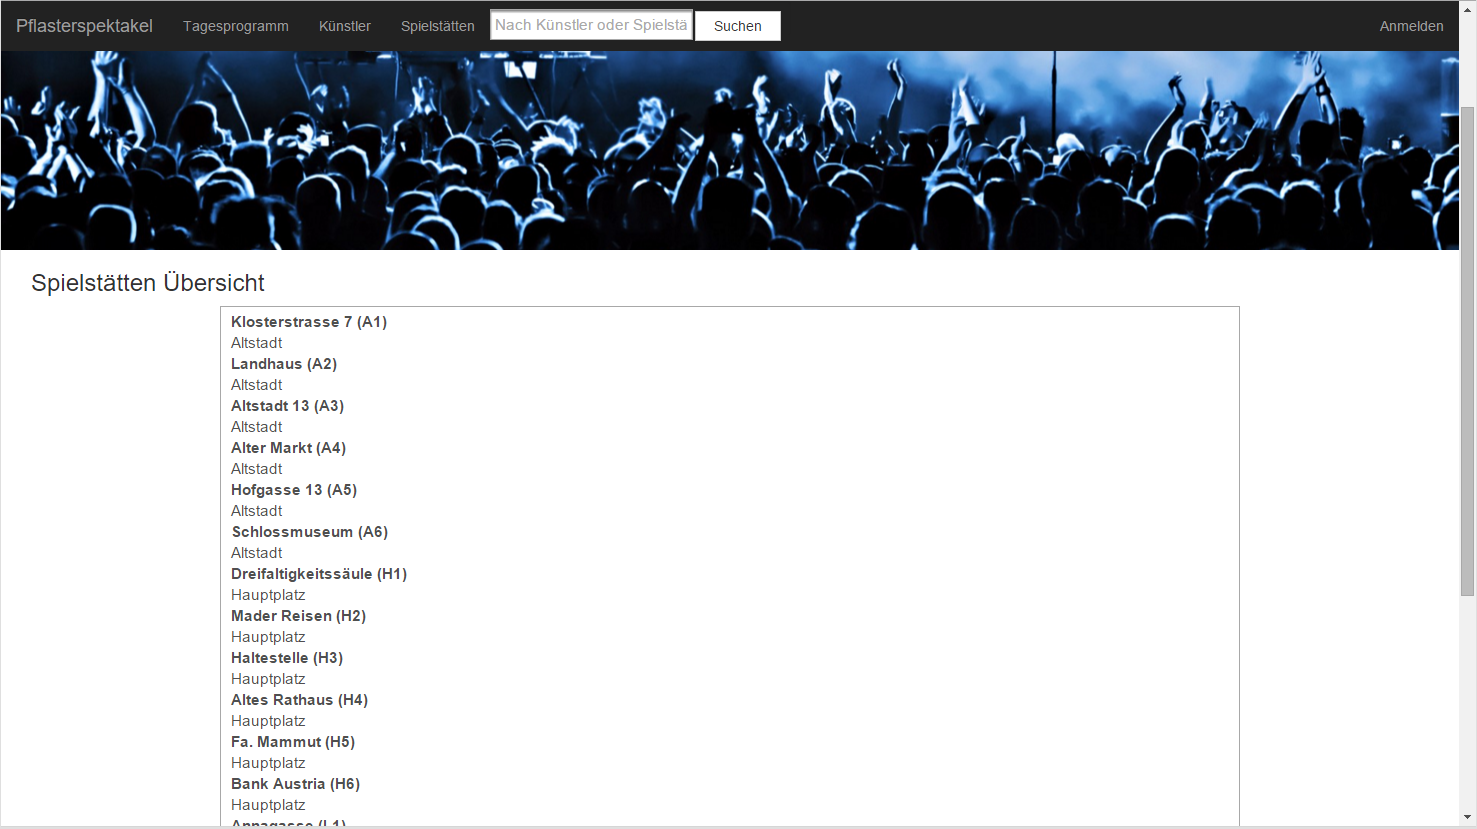
\includegraphics[angle=0, scale=0.40]{./img/3_ausb_page4.PNG}
\FloatBarrier
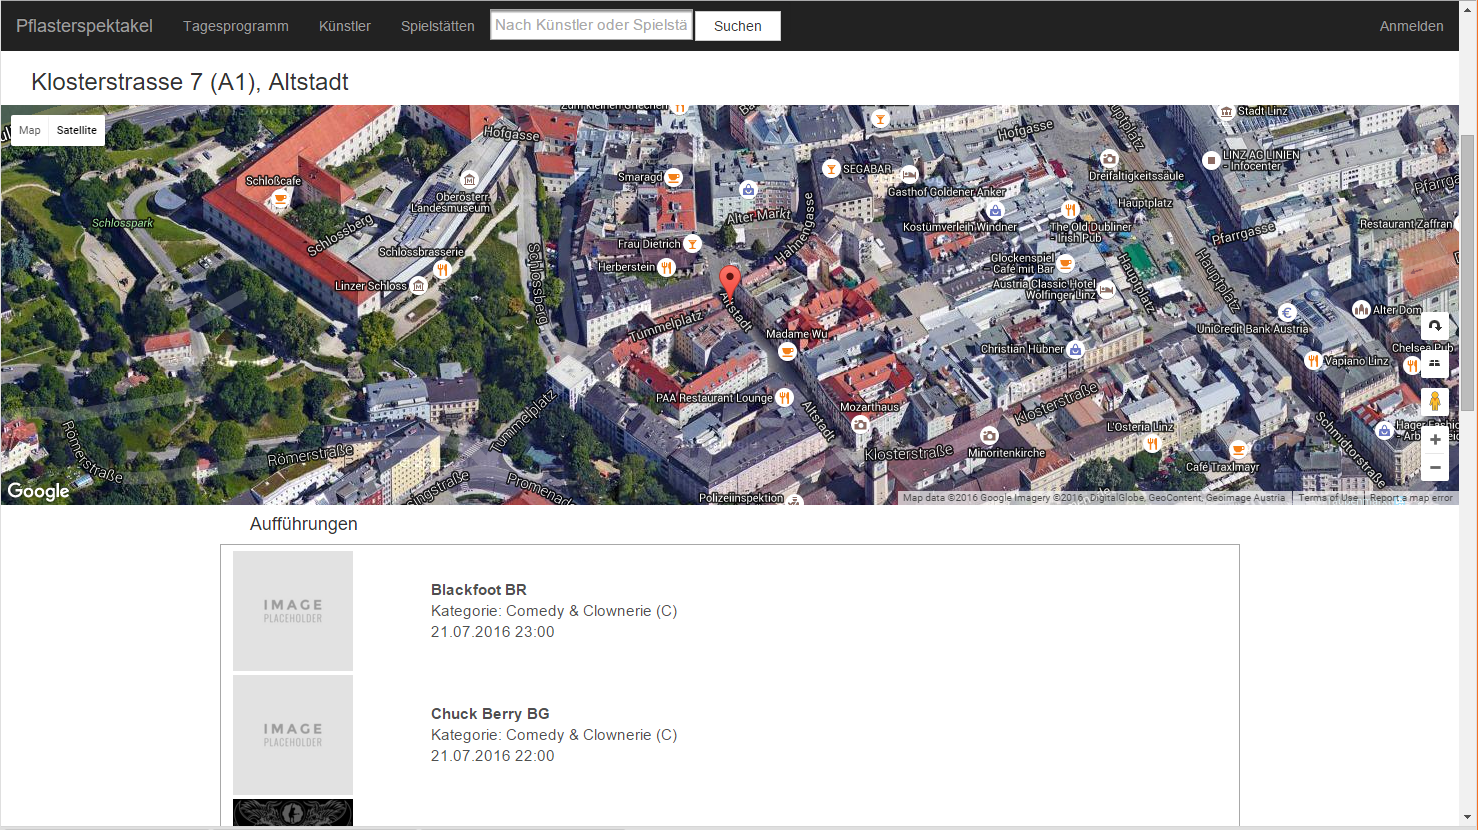
\includegraphics[angle=0, scale=0.40]{./img/3_ausb_page5.PNG}
\FloatBarrier
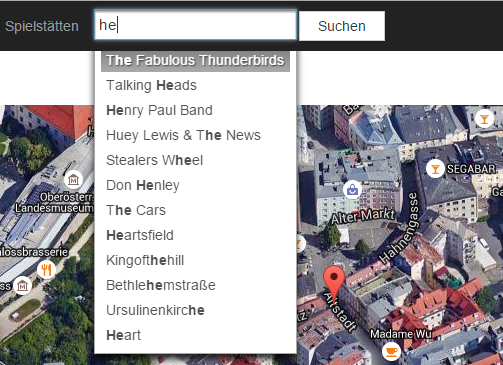
\includegraphics[angle=0, scale=0.65]{./img/3_ausb_page6.PNG}
\FloatBarrier
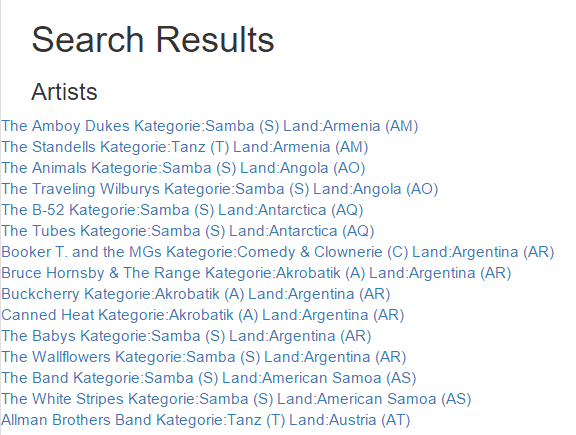
\includegraphics[angle=0, scale=0.65]{./img/3_ausb_page7.PNG}
\FloatBarrier

\end{section}